\documentclass{article}
\usepackage[utf8]{inputenc}
\usepackage[english]{babel}
\usepackage{amsmath}% http://ctan.org/pkg/amsmath
\usepackage{listings}
\usepackage{graphicx}
\usepackage{comment}
\usepackage{float}
\usepackage{biblatex}
\usepackage{lscape}
\usepackage{csquotes}
\usepackage{multirow}
\usepackage{float}
\usepackage{caption}

\addbibresource{bibliography.bib}
\usepackage[a4paper,pdftex,bottom=20mm, width=160mm]{geometry} % A4paper margins
\setlength{\parindent}{0pt} % Tar bort indenteringen på paragrafer 
\setlength{\parskip}{1em}

%tar bort linebreaks "i ord"%
\tolerance=1
\emergencystretch=\maxdimen
\hyphenpenalty=10000
\hbadness=10000
%------%

%Integration of Git for version control%




\title{
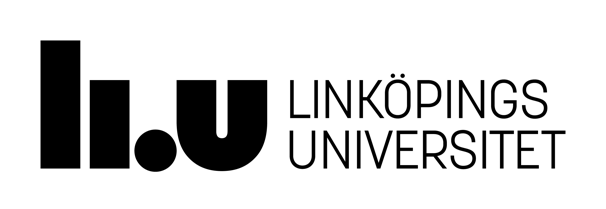
\includegraphics[scale=1.5]{liu_logga.png} \\
\vspace{2.0cm} \textbf{Customer Requirements Specification} \\
 \endgraf\rule{\textwidth}{.4pt}
  \large \textbf{TDDC88 - Project}\\
 
   }
   
   
\author{William Eriksson, Alina Wåhlberg, Gustav Gaunitz \& Melker Forsberg}

\date{\today} 

\begin{document}

\maketitle


\newpage
\tableofcontents
\newpage

% Here you will find information about the file
\section{Introduction}


\subsection{Purpose}
The purpose of this Customer Requirements Specification is to define the customer’s needs and expectations for the development of the system. It serves as a basis for communication between the customer, developers, and stakeholders, ensuring that all parties have a common understanding of the project’s objectives and scope. The document will guide the system's design, implementation and testing in accordance with the IEE standard 830-1998.


\subsection{Scope}

The project is conducted by 27 students from Linköping University taking the course "TDDC88" working in collaboration with Axis Communications. The project group, from here on called Company 3, consists of students with diverse educational backgrounds, including industrial engineering, computer science, and information systems analysis. The goal of the project is to create a functional system integrating Axis communications surveillance cameras and speakers with a easy to use UI which shall be tailored for a security company. The goal for the end customer is to protect facilities in a cost effective manner. 



\subsection{Definitions, acronyms and abbreviation}

This section provides an overview of the user roles within the system and their overall purpose. It also includes a list of abbreviations relevant to understanding the requirements in this document.

\subsubsection{User roles}
This subsection describes the user roles for the system. They are built on each other, meaning as you move up the access hierarchy, with the latter ones meaning more access, you gain more features in the system. The manager and admin role may overlap depending on the customer's preferences.
 \begin{itemize}
    \item 
    \textbf{Guard:} Lowest level of access, shall receive notifications in case of an approved alarm and then view the details of the alarm including a snapshot through a link in said notification. No actual input or further access to the system is given.
    \item 
    \textbf{Operator:} The operator class implies on the ones surveying the system constantly. They should be notified when the system detects a potential intruder and then be able to make an informed decision based on the snapshot and either approve or dismiss alarms. Operators are also allowed to cancel active alarms.

    \item \textbf{Manager:} Managers adds the functionality of viewing statistics of triggered alarms in order to take informed decisions on e.g. staff planning and camera locations. No further control of the actual alarms than the operators.

     \item 
    \textbf{Admin:} Administrators add the functionality of controlling camera and system parameters. These include camera controls such as brightness and system parameters such as required confidence level to trigger the system.

\end{itemize}

\subsubsection{Abbreviations}

\begin{itemize}
   \item \textbf{ACAP:} Axis Camera Application Platform, "An open application platform for software-based solutions built around Axis devices." \cite{ACAP}
     \item \textbf{GDPR:} General Data Protection Regulation,
"This regulation sets out provisions regarding the protection of natural persons in relation to the processing of personal data and the free movement of such data." \cite{GDPR}
\end{itemize}

\newpage

% Here you'll find information about the project
\section{Overall Description}

\subsection{Product perspective}

\subsubsection{User Stories}

User stories are ranked using priority and estimate. Priority 
indicates the significance or priority of a user story, assisting the team in determining which features to address first according to business objectives or stakeholder demands. Difficulty 
refers to the amount of work or time required to complete a user story, commonly measured in story points or hours, helping with planning and resource distribution.

 \begin{itemize}
    \item As an \textbf{Operator}, I want to be able to make an informed decision when an alarm is triggered by the system, giving me a snapshot of the situation, in order to ensure that the external alarm, including the speaker, is only triggered in actual intruder situations. \textbf{(Priority: 5, Difficulty: 3)}
    
    \item As an \textbf{Operator}, I want to be able to turn off the external alarm when a situation is resolved, in order to restore surveillance of the area and allow the system to add the event to the statistics database. \textbf{(Priority: 5, Difficulty: 2)}
    
    \item As an \textbf{Administrator}, I want to be able to configure the system with settings in terms of scheduling when the alarm should be active and the confidence intervals for the cameras, in order to adjust it to suit the specific area of surveillance. \textbf{(Priority: 4, Difficulty: 3)}
    
    \item As an \textbf{End Customer}, I want the system to be intuitive to use, in order to operate it with minimal technical training. \textbf{(Priority: 4, Difficulty: 3)}
    
    \item As a \textbf{Manager}, I want to get a visual representation of the data collected by the system, including triggered alarms, dismissed alarms, and triggered external alarms, in order to optimize staffing levels, adjust camera placement, and scheduling accordingly. \textbf{(Priority: 3, Difficulty: 3)}
    
    \item As a \textbf{Guard}, I want to receive a clear notification when an alarm has been approved that specifies where I am expected to go and what I can expect to encounter, in order to prepare for the situation and know exactly where to go. \textbf{(Priority: 4, Difficulty: 2)}
\end{itemize}


\subsection{Product functions}
The system will use the Axis camera and speaker to identify potential intruders. The software that will be developed will enable users to access different functionality such as alerts, camera settings and visual dashboards of the history. The concrete functions of the system will be: 

\begin{itemize}
    \item \textbf{Object Recognition:} The system shall recognize and classify objects in motion with a confidence level presented as a percentage. This feature uses advanced image processing algorithms built into the cameras to identify objects and determine their types.
    \item \textbf{Alerts to Operator:} Upon detecting a potential threat, the camera system will generate an alert that will be sent to the active operator. This alert includes sending images/videos, location and timestamp to the operational system and triggering an alarm if the threat is confirmed.
    \item \textbf{Alerts to Database:} Upon creating an alert, the timestamp, image/video, location and camera ID will be sent to the database.
    \item \textbf{Alarm Management:} Operators will have the ability to manage alarms by turning on or off the alarm system, including the speaker, and will have the option to confirm or deny the alarm based on the assessment of the displayed threat.
    \item \textbf{Scheduling Management:} Admin users will be able to configure and update the camera schedule. This function allows for flexible scheduling to ensure optimal camera coverage.
    \item \textbf{Confidence Adjustment:} Admin users will be able to adjust the camera’s confidence level. This allows for fine-tuning of the object recognition system to improve accuracy.
    \item \textbf{Live Camera Feeds:} Operators will have access to live feeds from active cameras, including their locations, to monitor real-time activities.
    \item \textbf{User Interface Navigation:} The system will provide an intuitive interface for operators to navigate through active camera feeds and manage alert responses effectively.
    \item \textbf{Alert Visualization:} Managers will have access to visual representations of alerts as data points, including the number of alerts, their locations, and timestamps. This data will be displayed in diagrams for easy analysis.
    \item \textbf{Alert Notifications Operator:} The system will visually indicate when an alert occurs through pop-ups or window changes, ensuring that operators are promptly informed.
    \item \textbf{User Management:} The system will support multiple user categories (Guard, Operator, Manager, Admin) with different access levels and capabilities. This includes the ability to manage user permissions and roles.
    \item \textbf{Integration and Accessibility:} The system will include standard pages such as login, user profile management, and system configuration to ensure ease of use and accessibility for authorized users.
\end{itemize}

\subsection{General constraints}
Since Company 3 consists of 27 employees from with varying competences, it requires effective coordination and task allocation to leverage the specialized knowledge of each discipline. Furthermore one can assume that a significant amount of the time budget must be used on educating employees on areas of lacking expertise. 

The aforementioned time budget, presenting the largest constraint, of the project, is a strict limit of 160 hours per employee. This necessitates efficient time management, prioritization of tasks, and the implementation of streamlined processes to ensure that the project is completed within the available time frame. 

The nature of the company operating withing the boundaries of a university course create other certain time constraints that the company must adhear to. This includes strict deadlines of iterations, pre-planned meetings, assignments e.tc. which limit the possibility of true to life operations and consumes a portion of the total time budget. 

\subsection{Assumptions and dependencies}
The following assumptions have been made of the system, its users and customers:

\subsubsection{Limitations of user classes}
Users accounts are limited to one type of access level e.g. guards cannot be administrators. We remove this need by structuring higher levels of access as containing all features of lower ones i.e. building upon each other. 

\subsubsection{Installation of cameras and networking}
Company 3 delimits itself from responsibility in any part of either the installation of the cameras nor the networking that would be needed for application for a end-customer. The construction of the system will take little to no regard to ease of first installation, instead focusing on the usability of a pre-installed system.

\subsubsection{Staff planning}
The system shall provide the manager statistics to create cost effective staff planning. Company 3 provides the statistics and dashboard but delimits itself from gathering insights from these.

\subsubsection{Dashboard monitoring}
Company 3 assumes that the dashboard of the system will be monitored constantly by the end customers staff to take informed decisions on the alarms. This means that we will not send automatic notifications to guards in case of a lack of action on triggered alarms.

\subsection{Lower ambition levels}
To manage risks related to the time budget or other resource constraints, certain features or goals of this project may be considered for reduction or deferral. Hopefully without significantly impacting the core functionality or overall success of the system. The following areas are identified as candidates for scope reduction:

\subsubsection{Non-essential features}
Certain functionalities that enhance the user experience or provide additional capabilities, but are not critical to the system's primary operations, may be postponed or excluded from the initial release. 

Specific examples include the mobile version of the web application which could be omitted for more detailed notifications, as approved  by AXIS, relieving mainly front-end work. Furthermore the refinement of the UI is a typical case where function over form can become the norm if budget constraints arise.

\subsubsection{Performance optimization}
Enhancing the performance of a system should always be a goal of development, however minimum acceptable standards could be adjusted to meet budget constraints. Further refinements could instead quite easily be addressed in future iterations of the system.

\subsubsection{Non-critical testing}
Non-critical testing scenarios, such as edge cases or performance stress testing beyond expected operational loads, may be reduced to focus on core functional and usability testing.

\newpage

% Here you'll find information about requirements
\section{Specific requirements}

\subsection{Interface Requirements}
The system shall provide an interface which makes it easy to use and access. In order to achieve this the system shall have a cohesive graphic design when it comes to font, font size, header size, color scheme, page structure etc. The system shall have an interface which is intuitive to use such as standard pages in the application, i.e. login page, change information, start page and so on. Additionally, the user shall also be able to orient into active camera feeds and to dashboards presenting statistics. 


\subsection{Functional Requirements}
The system provides different functionality depending on the access level of the current user. User types follow a hierarchical structure, where each successive level grants increased access compared to the one before. The top role, admin, will have full access to the system. This will allow managers to set up new accounts, add cameras, adjust scheduling and adjust access. 

The camera will detect objects in motion, and based on the current confidence level and selected threat types, an alert will be sent to the operator. The camera will also record  timestamp, location, and capture a snapshot or video, which will be stored in a database. The operator will assess the alert and determine the appropriate course of action. If the alert is confirmed as a genuine threat, it will be marked as "verified" which triggers an alarm. For verified threats, the operator will notify a guard providing them with the timestamp, location, and key imagery from the incident. 

The system will include a page dedicated to displaying statistics, accessible by the supervisor. This page will retrieve data from the database and display the number of alerts, their locations, and timestamps in a diagram. 
\clearpage
\begin{table}[h] 
\centering
\begin{tabular}{|l|p{8cm}|p{5cm}|}
\hline
\textbf{ID} & \textbf{Description} & \textbf{Implementation Plan} \\
\hline
FRQ001-v1 & The camera system shall recognize objects in motion and define what they are with a confidence presented as a percentage. &  \\
\hline
FRQ002-v1 & The camera system shall send images and videos to the operational system if it is triggered. &  \\
\hline
FRQ003-v1 & The operational system shall alert the operator of an intrusion within 5 seconds of detection. &  \\
\hline
FRQ004-v1 & The operational system shall enable the operator to turn off the alarm (including the speaker) at any time. &  \\
\hline
FRQ005-v1 & The operational system shall display the option for an operator to either confirm or deny an alarm. &  \\
\hline
FRQ006-v1 & The admin shall be able to update the camera schedule within 10 minutes. &  \\
\hline
FRQ007-v1 & The admin shall be able to update the camera’s confidence within 10 minutes. &  \\
\hline
FRQ008 & The operator shall be able to see active cameras and their locations live. &  \\
\hline
FRQ009-v1 & The operator shall be able to orient into "active camera feeds". &  \\
\hline
FRQ010-v1 & The managers shall be able to see the number of alerts in a diagram. &  \\
\hline
FRQ011-v1 & The managers shall be able to see the location of the alerts in a diagram. &  \\
\hline
FRQ012-v1 & The manager shall be able to see the time of the alerts in a diagram. &  \\
\hline
FRQ013-v1 & The system shall visually show the operator when an alert is occurring (e.g., popup, change window). &  \\
\hline
FRQ014-v1 & The system shall have 4 different "user" categories, with different access levels. (Guard, Operator, Supervisor, Admin) &  \\
\hline
FRQ015-v1 & The guard shall be alerted if the operator approves the alarm on a mobile unit. &  \\
\hline
FRQ016-v1 & The operator shall manage and assess the alarms. &  \\
\hline
FRQ017-v1 & The supervisor shall be able to see statistics and alarm analysis. &  \\
\hline
FRQ018-v1 & The admin shall be able to configure the system and manage the users and their access levels. &  \\
\hline
\end{tabular}
\captionsetup{justification=centering}
\caption{Functional Requirements for the Camera System, implementation plan will be decided later on in the project in collaboration with the architect and developers}
\label{table:functional_requirements}
\end{table}

 




\subsection{Performance requirements}
The system shall have a database storing data connected to triggered alarms including date, time, location and a comment. It shall also store private information including snapshots in accordance to GDPR regulations.

    The admin shall be able to schedule when the cameras will be active and inactive and this shall compile within a reasonable amount of time.  It shall also be possible for the admin to update the confidence level in the cameras without a noticeable delay in the system.   

\begin{table}[h!]
\centering
\begin{tabular}{|l|p{8cm}|p{5cm}|}
\hline
\textbf{ID} & \textbf{Description} & \textbf{Implementation Plan} \\
\hline
NRQ001-v1 & The database shall store private information, including snapshots, in accordance with GDPR regulation. &  \\
\hline
NRQ002-v1 & The database shall store data about triggered alarms, including date, time, location, and a comment. &  \\
\hline
NRQ003-v1 & The admin shall be able to update the camera schedule 95\% of the time. &  \\
\hline
NRQ004-v1 & The admin shall be able to update the camera confidence 95\% of the time. &  \\
\hline
NRQ005-v1 & The user interface shall be intuitive to use. &  \\
\hline
NRQ006-v1 & The system shall have a cohesive graphic design (Font, Font size, header size, color scheme, page structure). &  \\
\hline
NRQ007-v1 & The system shall use a login portal to adjust accessibility through account settings. &  \\
\hline
\end{tabular}
\captionsetup{justification=centering}
\caption{Non-Functional Requirements for the Camera System, implementation plan will be decided later on in the project in collaboration with the architect and developers}
\label{table:nonfunctional_requirements}
\end{table}

\clearpage


\subsection{Design constraints}
The design within the application will compile with the color scheme and other details from the first drafts for the authentication-page and dashboard as seen in \ref{fig:authenticationPageFirstDraft} and \ref{fig:dashboardPageFirstDraft}. \\

\begin{figure}[H]
    \centering
    \topmargin = 20pt
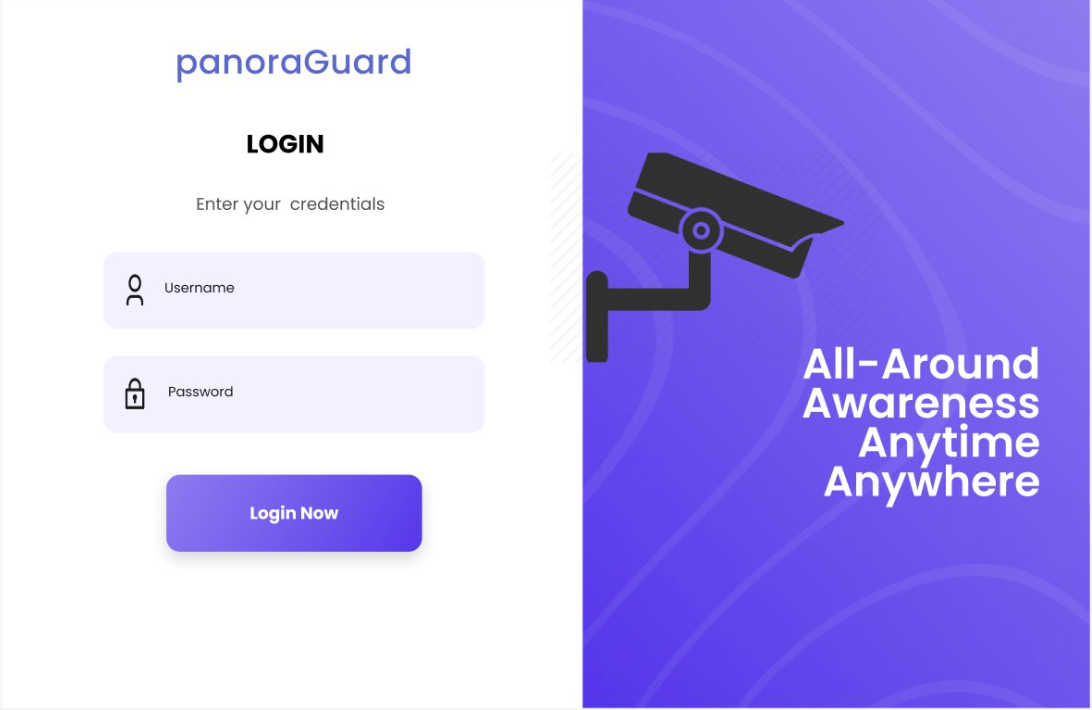
\includegraphics[width=0.75\linewidth]{authenticationPageFirstDesignDraft.png}

    \caption[width=0.75]{First draft of the visual design for the authentication page.
    }
    
    \label{fig:authenticationPageFirstDraft}

    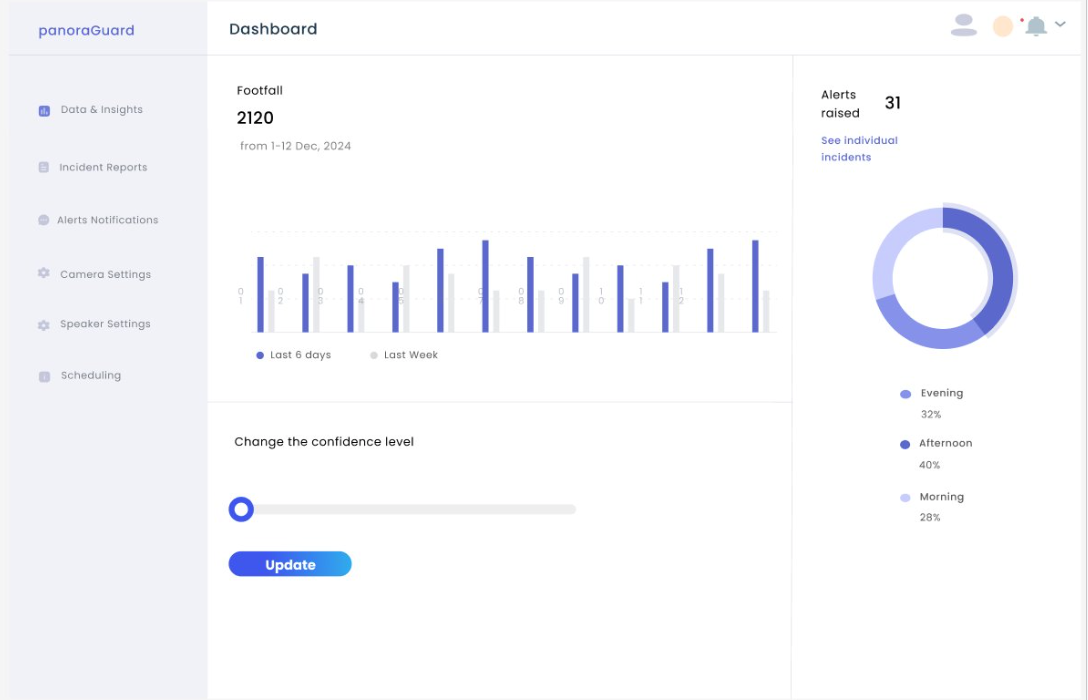
\includegraphics[width=0.75\linewidth]{dashboardFirstDesignDraft.png}
    \caption[width=0.75]{First draft of the visual design for the dashboard page presenting various kinds of statistics.}
    \label{fig:dashboardPageFirstDraft}
\end{figure}


\subsection{Software system attributes}
This part should focus on the systems handling power and attributes. For example how many active users, how easy it is to incorporate and use, code standards and so on. \textbf{Will be most useful if the developers decide this so ask Chioma.} 


\newpage
¨% Here you'll find additional relevant info about the project


\newpage
\printbibliography

\end{document}
